\documentclass{UoYCSproject}
\addbibresource{REFERENCES.bib}

\usepackage{tikz}
\usetikzlibrary{automata, positioning, arrows}

\usepackage{float}

\usepackage{graphicx}

\usepackage{listings}

\tikzset{
  ->, % makes the edges directed
  node distance=4cm, % specifies the minimum distance between two nodes. Change if necessary.
  every state/.style={thick, fill=gray!10}, % sets the properties for each ’state’ node
  initial text=$ $, % sets the text that appears on the start arrow
}

\newenvironment{monospace}{\ttfamily\small}{\par}

\BEng
\supervisor{Dr. Christopher Crispin-Bailey}

\dedication{}

\acknowledgements{
I would like to thank my supervisor, Dr. Chris Crispin-Bailey, for his guidance throughout this project.
}

\begin{document}

\title{Generation of Hardware Accelerators for an FPGA System}
\author{Jay Valentine}

\maketitle

\begin{abstract}
With the increase in market share of embedded general-purpose computing platforms such as mobile phones
and tablets, energy efficiency is of increasing concern. One obstacle to achieving energy efficiency
at the transistor scales of todays devices is dark silicon, a phenomenon which limits the percentage
of a chip that can be utilized at any one time.

Coprocessor-dominated architectures are a solution to the dark silicon problem which have recently been
gaining attention. However, traditional coprocessor models rely heavily on human-designed hardware accelerator
cores, the design of which is expensive and time-consuming. In addition, once implemented these coprocessors
are fixed, and so must be designed with a range of applications in mind. 

This report outlines a coprocessor-dominated architecture that can be implemented on an FPGA, based on the Xilinx
MicroBlaze soft processor. This allows for the architecture to be changed with the application demands.
In addition, a method is described (and a toolchain implemented) for transforming a basic block in the software application into
a specialized hardware accelerator core, custom-built for executing that specific basic block. This method can be completely
automated, reducing design costs and time.

Several architecture configurations generated with the tool were evaluated on two benchmark applications, intended to be
representative of embedded workloads. This evaluation showed improvements in both application performance and energy efficiency.
\end{abstract}

\chapter{Introduction}

\section{Motivation}

With the breakdown of Dennard scaling and the observation of dark silicon in modern microprocessors,
we are rapidly approaching a utilization wall, meaning that not all transistors on a given chip can be utilized
simultaneously \cite{darksilicon}. This has severe consequences for the future of microprocessor architecture,
especially in domains where energy consumption is of great concern, such as the rapidly growing mobile application domain.

Because of this, research is turning towards novel architectures as a solution to this problem.
One such architecture is the \textit{coprocessor-dominated architecture} (\textit{CoDA}), in which one or more general-purpose
processing cores are coupled with a large number of specialised hardware accelerators, which are able to perform very specific
tasks with greater energy efficiency than a general-purpose core.

\section{Aims}

This work aims to show that such an architecture can be utilized in an embedded FPGA platform.
The use of an FPGA allows the accelerators to be designed specifically with the embedded application in mind.
The aim is to produce a tool that can generate hardware accelerators from an application written for the Xilinx MicroBlaze
soft processor \cite{microblaze}.

Because the accelerators are automatically generated by the tool, rather than designed by hand, the architecture
can be re-generated for each version of the application, or even across different applications, very easily.
The use of an FPGA allows the architecture to be very highly specialized, as the FPGA can be re-programmed for each architecture
version. In this sense, the architecture itself becomes an extension of the application software, rather than a static
platform as has traditionally been the case.

\section{Statement of Ethics}

Neither the undertaking of this project, nor its end result, are envisioned to cause any harm. The end result is
a general-purpose computing platform, and while such a platform can certainly be used to cause harm, this is not an intrinsic
property of the platform, and this platform is no more suited to such a pursuit than any other computing platform.
All testing was automated and performed entirely using software tools; no personal data was collected nor were humans
or animals participants in testing in any way.

Some portions of code used as test applications in the evaluation of this system were sourced
from authors who had released the code as open source. Great care was taken to ensure that all
code used for this purpose was credited properly and that the licenses with which the code was
provided permitted its use in this project.

\chapter{Literature Review}

\section{Moore's Law and Dennard Scaling}

In 1965, Gordon Moore predicted that the number of transistors in an integrated circuit will double
approximately every two years  \cite{moore}. Similarly, Dennard scaling describes the way in which transistor power density
remains constant as the transistors themselves shrink in size \cite{dennard}. These phenomena combined allow for exponential
transistor-density increases, and this has been exploited to produce exponentially higher performance in
microprocessors year on year.

\begin{figure}[h]
\center{\includegraphics[width=\textwidth]
{figures/moore.png}}
\caption{Moore's 1965 prediction. \cite{moore}}
\end{figure}

However, in more recent times, a breakdown in this scaling has been observed. In the past, Dennard scaling has allowed
microprocessor manufacturers to offset the increased energy cost of faster transistor switching, resulting in higher
and higher clock speeds. However, more recently, microprocessor clock speeds have remained relatively static. This is
due to a breakdown in Dennard scaling for very small transistors, and has caused microprocessor manufacturers to instead
pursue increased performance by the use of multicore designs.

\begin{figure}[h]
\center{\includegraphics[width=\textwidth]
{figures/cpu-speed.png}}
\caption{Trends in microprocessors since 1970. \cite{karlrupp}}
\end{figure}

\section{Dark Silicon}

Dark silicon is a phenomenon which has been observed as transistor density in microprocessors has increased.
It occurs as transistor under-utilization leads to a gap between the speedup observed and that predicted by
extrapolating from historic performance gains.

In \cite{darksilicon}, it is predicted that with 22nm transistors, 21\% of the chip will be dark silicon,
with this rising to 50\% at 8nm. This prediction shows that dark silicon will become a serious limitation
as transistor density grows, especially in areas where energy efficiency is a primary concern.

Dark silicon also becomes a limiting factor with manycore devices. Even when energy consumption is not a
concern, the limited parallelism of most applications results in a dark silicon gap when running with
manycore devices. Again, \cite{darksilicon} shows that beyond a certain number of cores the speedup achieved
is negligible. This is another kind of dark silicon - the underutilization in this case is not a result of
energy concerns but is caused by the limited parallelism of the application being unable to exploit all of
the cores of a device.

There have been several broad responses to this phenomenon.
In \cite{four-horsemen}, Taylor gives two pessimistic predictions regarding the future of silicon
utilization. The first, the 'shrinking horseman', predicts that chips will begin to shrink as a result of
the utilization wall. This would lead to an increase in cost per mm\textsuperscript{2} of silicon, as
design costs, test costs, marketing costs, etc. Put simply, "exponentially smaller chips are not
exponentially smaller".

The second, perhaps slightly less pessimistic, prediction in Taylor's paper
is referred to as 'the dim horseman', and describes the under-clocking or infrequent use of
general-purpose silicon in order to meet power budgets. While a better alternative than the shrinking
of chips, this still causes issues as the chip is no longer operating at maximum capacity.
Taylor outlines several options for the use of this 'dim silicon'. The first, and perhaps most obvious,
is the use of homogenous architectures, but with some cores operating at a lower clock speed, or
even being turned off intermittently. However, there are other 'dim silicon' approaches that make better
use of the unutilized silicon area. One approach is to increase cache sizes, as cache memory is less
power-dense than a processing core would be. This has a secondary benefit as well, in that a larger
cache will reduce the number of cache misses, thereby decreasing the number of power-hungry off-chip
accesses.

Finally, Taylor also describes 'the specialized horseman'. This approach is to use the dark silicon area
not for general-purpose computing, but for a large number of specialized cores, which would be much
more energy efficient than a general-purpose core, allowing for increased energy efficiency at the
cost of silicon area.

\section{Heterogeneous Architectures}

One such 'specialized horseman' approach is the use of heterogeneous architectures.
These are computer architectures in which one or more general-purpose cores are coupled with special-purpose coprocessors,
also known as hardware accelerators. A hardware accelerator is a specialised hardware circuit intended to perform a
specific task more efficiently than a general-purpose processor. While historically hardware accelerators have been designed by
hand for a specific application (e.g. encryption), this is infeasible when considering architectures
with large numbers of accelerators. Thus an automated approach to generating hardware accelerators is required.

This is the approach taken in \cite{high-performance-microarchitecture}. Here Razdan and Smith propose a simple
hardware accelerator architecture which avoids the need for memory synchronization and reduces the overheads involved in
invoking a hardware accelerator. They describe a toolchain which is able to extract instruction streams to be 'outsourced' to an
accelerator core (called a \textit{programmable functional unit}, or \textit{PFU}) after code generation.

\begin{figure}[hbt]
\center{\includegraphics[width=0.75\textwidth]
{figures/pfu.png}}
\caption{Two PFU optimization examples. Both sequences of operations can be evaluated in a single cycle, while the same sequences in MIPS R2000 instructions would take multiple cycles. \cite{high-performance-microarchitecture}}
\end{figure}

The PFU model is a simplification from the general model of a hardware accelerator, which is as a multi-cycle state machine.
Instead each PFU has at most two input operands and at most one output operand. In addition, the PFU-logic instructions (MIPS
instructions that are candidates for translation into a PFU) cannot be memory-access or flow control instructions. This means
that each PFU has an identical interface, and can be executed in a single cycle. This allows PFUs to be executed with a single
instruction, \textit{expfu}, in a single cycle, maintaining the fixed-format and single-cycle instructions of the MIPS
processor's RISC instruction set.

\section{Conservation Cores}

While traditionally hardware accelerators have been used to speed up certain computations, they can also be used to achieve the
same computational performance as a general-purpose processor at a fraction of the energy cost, thus alleviating the dark silicon
problem.

\cite{c-cores} introduces \textit{conservation cores} (\textit{c-cores}), which are hardware accelerators
designed for this purpose. The paper outlines a method for generating c-cores for a given application.
The first step is to identify 'hot' and 'cold' portions of the application, using some form of profiling.
'Hot' code sections are those which are run frequently, and so are ideal candidates for c-cores. 'Cold' sections
are run infrequently, and so are not ideal candidates, as the overhead involved in using a c-core would
not be offset by the computation avoided by its use.

Once 'hot' portions are identified, a c-core can be synthesised for it. While previous hardware accelerators
might have been hand-designed, such an approach is not viable if large numbers of c-cores are to be used, and so
the paper outlines a method for automating the synthesis of these cores. A control-flow graph can be extracted
from the code, and from this a state machine model can be constructed to perform the functionality represented
in the code. This state machine can then be implemented in a language such as VHDL or Verilog, and from this a circuit
can be synthesised.

\begin{figure}[h]
\center{\includegraphics[width=\textwidth]
{figures/c-cores.png}}
\caption{Conservation core example. \cite{c-cores}}
\end{figure}

One of the main issues with these c-cores is that memory synchronization restricts ILP (instruction-level parallelism)
and requires large numbers of pipeline registers (as each memory access marks a state-boundary). \cite{eco-cores} attempts
to alleviate this issue by introducing \textit{selective de-pipelining} (SDP), in which memory accesses occur in 'fast states'
while the rest of the processing done by the c-core proceeds as before, in 'slow states'.

Signals can safely propogate through the entire block without the need for latching on fast-state boundaries,
while values loaded from memory are latched on fast-state boundaries as soon as they are available.
An example of this process is shown in figure 2.4.

\begin{figure}[h]
\center{\includegraphics[width=\textwidth]
{figures/sdp.png}}
\caption{Selective de-pipelining example. \cite{eco-cores}}
\end{figure}

The GreenDroid project \cite{greendroid} takes the ideas of both \cite{c-cores} and \cite{eco-cores} and attempts
to apply them to the Android operating system and software stack. Mobile phone processors have vastly lower power budgets than
traditional desktop processors, both to achieve long battery life and to reduce generated heat. Profiling of the Android
software was used to identify the best portions of code to be converted into c-cores. As a result,
c-cores account for over 90\% of execution time, and if clock-gated when not in use (leaving them idle and consuming
very little power), this leads to a significant reduction in energy consumption.

A similar approach is taken by Arnone in \cite{arnone-thesis}. Here, Arnone outlines a method of
generating accelerator cores for a stack architecture, resulting in both timing
and power improvements. Two architectures for generated cores are described: composite and wave-core.
Composite cores are simple state machines with instructions mapped to states. Composite cores attempt to
optimise for logic area by reusing existing logic between states. Conversely, the wave-core
architecture avoids the reuse of logic between states, reducing power density at the cost of increased
logic area (due to potentially duplicated functionality). In both cases the resulting accelerator core is
more energy-efficient than the general-purpose processor is at the same task.

Here each core is a finite state machine generated from a basic block in the stack architecure's
assembly code. States are divided between computation states and memory-access states. Each computation state
is formed of a series of HDL (VHDL is used, but this could just as easily be Verilog) statements which are direct
translations of instructions in the stack architecture's instruction set. Between each computation state are one
or more states in which memory is being accessed, to either load or store data. Outputs from each state are latched
in registers so that they are available for the next state to operate on. Because each computation state is a simple
data-flow system with no need for synchronization, they can be completed within a single cycle.

These cores differ from conservation cores in that there is no control flow - while c-cores can encode loops, Arnone's
work focuses solely on basic blocks. This means that less use can be made of the cores (as the main processor must still
perform flow control), but also that the implementation of state machines is less complex - they are linear.

\chapter{System Design}

This chapter describes the architecture and design of the MicroBlaze system and the accelerator cores, and the
methods of communication between them. It also describes the methods used to analyse the object code in order to
extract accelerator cores, as well as the ways in which blocks to be extracted are selected automatically.

\section{System Architecture}

MicroBlaze \cite{microblaze} is a 32-bit RISC architecture, intended for implementation on an FPGA.
It is highly configurable, as certain features (e.g. FPU, multiplier, barrel shifter) can be disabled if not required.
This allows the architecture to be as minimal as is required by the application. Because of this, MicroBlaze is often used in
embedded environments where power efficiency is a significant concern.

The system used in this project consists of one MicroBlaze core, connected to local instruction and data block RAM (BRAM)
via the local memory bus (LMB). The processor's AXI bus is used to connect to a hardware-accelerator control unit, which is
in turn connected to one or more hardware accelerator cores, as well as to the BRAM via another LMB interface.
All communication with memory and with the MicroBlaze core by hardware accelerators is managed by the control unit.

\begin{figure}[H]
\center{\includegraphics[width=0.70\textwidth]
{figures/architecture.png}}
\caption{System architecture.}
\label{fig:systemArchitecture}
\end{figure}

This reduces the number of signals required, as the accelerators themselves can use a simplified memory interface to communicate
with the memory and the MicroBlaze core, rather than each having to separately implement the LMB and AXI protocols.
The complexity of the LMB and AXI protocols, which provide for arbitration between competing master cores, are not required,
as it is guaranteed that only one core (either an accelerator or MicroBlaze) will be executing at any one time.

The LMB is intended for connecting the MicroBlaze core to on-chip BRAM, for use as a local cache memory, with instructions
and data being stored in off-chip flash or DRAM. The system topology described above allows for a tiled architecture,
with each block containing a MicroBlaze core and several hardware accelerators. Each tile would have its own local memory,
with these memories being connected in turn (via some kind of cache interface) to the system-wide main memory. However,
this is beyond the scope of this project, which focuses on a single MicroBlaze core with associated accelerators,
and a single BRAM, with no main flash or DRAM.

To further simplify the design, the more advanced MicroBlaze features, such as the hardware multiplier, divider, and barrel
shifter, are deactivated. This not only simplifies the generated HDL, speeding up synthesis and simulation times, but also
reduces the pool of instructions that need to be translated (as hardware multiply etc. instructions no longer appear in
application code).

\section{Hardware Accelerator Architecture}

\begin{table}[H]
\centering
\begin{tabular}{ |p{3cm}|p{2cm}|p{8cm}| }
\textbf{Signal} & \textbf{Direction} & \multicolumn{1}{c}{\textbf{Description}} \\
CLK             & I                  & Clock signal. \\[0.05cm]
RST             & I                  & Reset signal. Active HIGH. \\[0.05cm]
SEL             & I                  & Block-select signal. Block is active when this is HIGH, and inactive when this is LOW. \\[0.05cm]
DONE            & O                  & Done signal. This goes HIGH once the state machine has finished its computation, and goes LOW when the state machine is reset. \\[0.05cm]
M\_RDY          & I                  & Memory-ready signal. Signals to the state machine that a memory transaction has completed. \\[0.05cm]
M\_RD           & O                  & Memory read strobe. Indicates that the state machine is reading a value from memory. \\[0.05cm]
M\_WR           & O                  & Memory write strobe. Indicates that the state machine is writing a value to memory. \\[0.05cm]
M\_ADDR         & O                  & Memory address. Address of word being accessed in memory. \\[0.05cm]
M\_DATA\_OUT    & O                  & Data out. Data written to memory is placed on this line. \\[0.05cm]
M\_DATA\_IN     & I                  & Data in. Data read from memory is placed on this line. \\[0.05cm]
IN\_Rxx         & I                  & One or more input register lines. Inputs to the state machine are written to these lines from the MicroBlaze core. \\[0.05cm]
OUT\_Rxx        & O                  & One or more output register lines. Outputs from the state machine are written to these lines from the state machine once it has finished computation. \\[0.05cm]
CARRY\_IN       & I                  & Carry signal input. Indicates the state of the carry flag at the start of the state machine's execution. \\[0.05cm]
CARRY\_OUT      & O                  & Carry signal output. Indicates the state of the carry flag at the end of the state machine's execution.
\end{tabular}
\caption{Hardware accelerator input/output signals.}
\label{table:acceleratorSignals}
\end{table}

Each hardware accelerator is modelled as a sequential state machine, with a sequence of states determined by the structure
of the code that the hardware accelerator is intended to replace. Each state machine block has a similar interface, as defined in
table ~\ref{table:acceleratorSignals}. All transitions between states are synchronous, performed on the rising edge of the CLK
signal.

There are four kinds of states in the hardware accelerator model. The start state, which is the state the accelerator is in
when activated, transfers inputs from the accelerator's register input ports into internal registers, for use during the
computation. The end state is the state the accelerator moves to when the computation is complete. In this state, output values
are transferred from the accelerator's internal registers to the register output ports, to be read by the MicroBlaze core.
An example abstract state machine is shown in figure ~\ref{fig:abstractStateMachine}.

\begin{figure}[H]
\centering
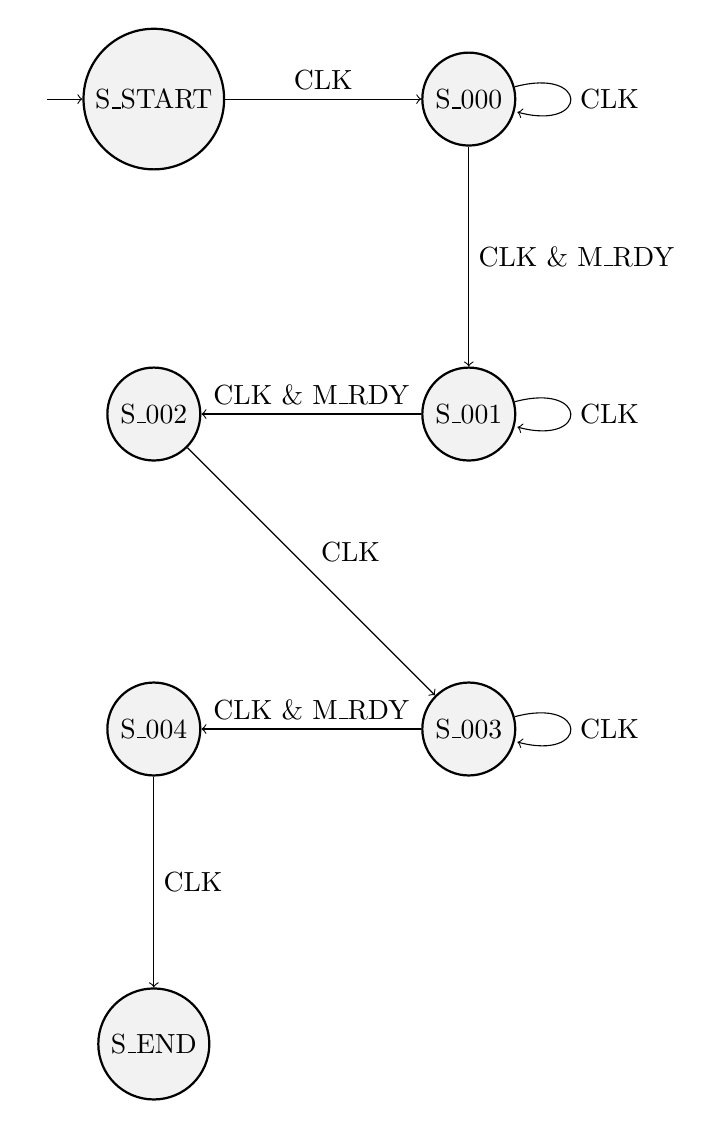
\begin{tikzpicture}
  \node[state, initial] (S_START) {S\_START};
  \node[state, right of=S_START] (S_000) {S\_000};
  \node[state, below of=S_000] (S_001) {S\_001};
  \node[state, left of=S_001] (S_002) {S\_002};
  \node[state, below of=S_001] (S_003) {S\_003};
  \node[state, left of=S_003] (S_004) {S\_004};
  \node[state, below of=S_004] (S_END) {S\_END};

  \draw (S_START) edge[above] node{CLK} (S_000);
  \draw (S_000) edge[loop right] node{CLK} (S_000);
  \draw (S_000) edge[right] node{CLK \& M\_RDY} (S_001);
  \draw (S_001) edge[loop right] node{CLK} (S_001);
  \draw (S_001) edge[above] node{CLK \& M\_RDY} (S_002);
  \draw (S_002) edge[above right] node{CLK} (S_003);
  \draw (S_003) edge[loop right] node{CLK} (S_003);
  \draw (S_003) edge[above] node{CLK \& M\_RDY} (S_004);
  \draw (S_004) edge[right] node{CLK} (S_END);
\end{tikzpicture}
\caption{An example abstract state machine.}
\label{fig:abstractStateMachine}
\end{figure}

In between the start and end states are a series of computation and wait states. A computation state is derived from a series of
non-memory-access instructions (e.g. \texttt{addi} (add-immediate) or \texttt{srl} (shift-right logical)).
A circuit is constructed from the instructions which implements the same functionality, but in parallel,
as shown in figure ~\ref{fig:computationState}. As such, while the instructions represented by a computation state might take
several cycles to complete on a general-purpose processor, the hardware accelerator can always complete a computation state in a
single cycle. The translations of MicroBlaze instructions used in the generation of accelerator cores can be seen in Appendix A.

\begin{figure}[H]
\center{\includegraphics[width=0.75\textwidth]
{figures/computation-state.png}}
\caption{Comparison of original program instructions and generated parallel circuit.}
\label{fig:computationState}
\end{figure}

Each computation state is separated by one or more wait states, in which the accelerator either fetches data from or writes data
to the local memory. Each wait state is associated with a single input/output instruction
(e.g. \texttt{lwi} (load word immediate) or \texttt{sb} (store byte)). These states can typically be completed within two
cycles, but may take more depending on memory latency.

\section{Accessing Cores}

In order for the generated hardware accelerators to be at all useful, a lightweight system to allow the MicroBlaze core to
activate them and retrieve results is required. The accelerator cores are connected, via a controller module, to the
general-purpose core via the AXI bus, which exposes the controller to MicroBlaze as a set of memory-mapped registers.
These registers can then be written to and read from using the \texttt{sw} (store word) and \texttt{lw} (load word) instructions.
Table ~\ref{table:controllerRegisters} shows the locations and purpose of these registers.

\begin{table}[H]
\centering
\begin{tabular}{ |p{6cm}|p{7cm} }
\textbf{Memory Location}   & \textbf{Description}        \\
HW\_ACCEL\_PORT            & Control register.         \\[0.05cm]
HW\_ACCEL\_PORT + 4        & I/O for register R1.      \\[0.05cm]
...                        & ...                       \\[0.05cm]
HW\_ACCEL\_PORT + 120      & I/O for register R30.     \\[0.05cm]
HW\_ACCEL\_PORT + 124      & I/O for MSR register.     \\[0.05cm]
\end{tabular}
\caption{Controller module memory-mapped registers. The symbol HW\_ACCEL\_PORT represents the memory location to which the controller is mapped.}
\label{table:controllerRegisters}
\end{table}

There is no memory-mapped register for R31 because R31 is reserved by the compiler for storing the MSR system register when
transferring it to and from the accelerator cores. This means that R31 will never be used by the application code, and so
can be safely assumed to never be an input or output of a basic block (and by extension, an accelerator core). The transfer
of MSR is necessary because this system register holds information required by some instructions, such as the carry flag,
and so needs to be available to accelerator cores to modify.

\subsection{Transaction Overview}

Before activation, the controller module is in the READY state, waiting for the MicroBlaze core to pass inputs and select
a core to be activated. The controller module remains in this state as the MicroBlaze core transfers inputs by writing to
the appropriate controller module register. Once all inputs have been transferred, the required core is activated by writing
its numeric ID to the special control register. The MicroBlaze core then goes into a 'sleep' mode (by executing a \texttt{mbar}
instruction) while the controller module activates the core. The controller then goes into the WAITING state.

Once the core has finished its computation, it signals the controller, which goes into the DONE state, and transfers any outputs
to the controller module. The controller then asserts the MicroBlaze core's wakeup signal, and the MicroBlaze core reads
the appropriate outputs from the memory-mapped registers. Finally, it reads from the special control register to reset the
controller and the accelerator core, and the controller again goes into the READY state. The result of this read contains
the MSR system register, the final output from the core. If necessary, the MicroBlaze core then writes the new value of MSR into
the system register.

\subsection{Using a Small-Data Pointer}

The MicroBlaze CPU has two dedicated small-data-area pointers, R2 and R13 \cite{microblaze-ref}.
A small-data area is an area of memory to which a pointer is held for the duration of an application,
allowing fast access to the region. Such a pointer can be used to hold the address of the controller module,
speeding up access to accelerator cores.

\begin{figure}[H]
    \begin{minipage}[t]{0.5\textwidth}
      \begin{monospace}
      \# Save temporary registers.

      swi    r12, r1, -4

      swi    r11, r1, -8
\\

      \# Get pointer to controller.

      addik  r12, r0, HW\_ACCEL\_PORT
\\

      \# Write registers.

      swi    rX, r12, (X*4)

      ...
\\

      \# Activate required core.

      \# C\_id is the core's

      \# numeric ID (0-indexed).

      addik  r11, r0, C\_id

      swi    r11, r12, 0
\\

      \# Sleep until woken.

      mbar   16
\\

      \# Read registers.

      lwi    rX, r12, (X*4)

      ...
\\

      \# Read control register.

      \# This resets the core.

      \# The value is discarded.

      lwi    r0, r12, 0
\\

      \# Restore registers.

      lwi    r11, r1, -8

      lwi    r12, r1, -4
      \end{monospace}
    \end{minipage}
    \begin{minipage}[t]{0.5\textwidth}
      \begin{monospace}
      \# Save temporary register.

      swi    r11, r1, -4
\\

      \# Pointer to controller

      \# is in R13.
\\

      \# Write registers.

      swi    rX, r13, (X*4)

      ...
\\

      \# Activate required core.

      \# C\_id is the core's

      \# numeric ID (0-indexed).

      addik  r11, r0, C\_id

      swi    r11, r13, 0
\\

      \# Sleep until woken.

      mbar   16
\\

      \# Read registers.

      lwi    rX, r13, (X*4)

      ...
\\

      \# Read control register.

      \# This resets the core.

      \# The value is discarded.

      lwi    r0, r13, 0
\\

      \# Restore register.

      lwi    r11, r1, -4
      \end{monospace}
    \end{minipage}

  \caption{Activating a hardware accelerator core, with (right) and without (left) a small-data pointer.}
  \label{fig:smallData}
\end{figure}

As demonstrated in figure ~\ref{fig:smallData}, no temporary register needs to be used to hold a
pointer to the controller, as the pointer is already stored in the small-data register R13.
This reduces the number of instructions required to control an accelerator core.

Without the small data area, two extra instructions are required to save and restore a temporary register,
and another is needed to set up the pointer to the controller. These three instructions are eliminated with the use of a small
data pointer. This might seem insignificant, but if accelerators are used frequently, the eliminated cycles could provide
savings in both time and energy.

\section{Code Analysis}

In order to identify the best candidates for extraction into hardware accelerators, some analysis needs to be performed.
The first step in this analysis is to break the instruction stream up into basic blocks. A basic block is a linear portion of
code, bounded at both ends by flow control instructions (e.g. branch or call instructions), or a label (indicating that this
portion of code is the target of a jump somewhere else in the program). These blocks can then be linked
together into a program-flow graph, in which all nodes are basic blocks, and all edges links between those blocks.
From this representation, some information about the individual blocks can be extracted.

\subsection{Inputs and Outputs}

It is possible to know what the inputs and outputs from a block are in isolation (with an input being any register that is read
before being written to in the block, and an output being any register written to at any point in the block). However, this leads
to very conservative results, as highlighted by figure ~\ref{fig:analysisNaiveApproach}. In the example, \texttt{r6} is used as a
temporary register, and according to the MicroBlaze ABI \cite{microblaze-ref} is discarded on returning from the function. If we
take the naive approach to identifying a block's outputs, this information is ignored and it is assumed that because \texttt{r6}
is written to, it must be an output of the block. In a real block, there may be many more temporary registers used, resulting in
the analysis reporting a large number of 'false outputs'.

\begin{figure}[H]
  \begin{center}
    \begin{minipage}{0.5\linewidth}
      \begin{monospace}
      lwi r3,r5,0

mul r6,r3,r3

addik r3,r6,20

rtsd r15, 8

inputs: r5

outputs: r3, r6

      \end{monospace}
    \end{minipage}
  \end{center}

  \caption{A naive approach to basic block analysis.}
  \label{fig:analysisNaiveApproach}
\end{figure}

In order to solve this problem, the analysis needs to take into account both how the registers are used (as defined by the
ABI) and the context in which the block exists (i.e. what blocks come before and after it).
The register descriptions, taken from the ABI, are shown in table ~\ref{table:abi}. R3 and R4 are used for returning values from
subroutines, and so must be outputs from a basic block (if written to) if that block is the last block in a subroutine
(i.e. the last instruction in it is a \texttt{rtsd} instruction). However, as R5 to R12 are volatile, they are not preserved
when returning from a subroutine (as they will be restored by the caller). Therefore, if they are written to in the last block
of a subroutine, they can be discarded as outputs.

\begin{table}[H]
\centering
\begin{tabular}{ |p{2cm}|p{3cm}|p{8cm}| }
\textbf{Register} & \textbf{Type} & \multicolumn{1}{c}{\textbf{Description}} \\
R0       & Dedicated    & Hardcoded 0. \\[0.05cm]
R1       & Dedicated    & Stack pointer. \\[0.05cm]
R2       & Dedicated    & Read-only small-data-area pointer. \\[0.05cm]
R3-R4    & Volatile     & Return values/temporaries. \\[0.05cm]
R5-R10   & Volatile     & Passing parameters/temporaries. \\[0.05cm]
R11-R12  & Volatile     & Temporaries. \\[0.05cm]
R13      & Dedicated    & Read-write small-data-area pointer. \\[0.05cm]
R14      & Dedicated    & Return address for interrupts. \\[0.05cm]
R15      & Dedicated    & Return address for subroutines. \\[0.05cm]
R16      & Dedicated    & Return address for trap (debugger). \\[0.05cm]
R17      & Dedicated    & Return address for exceptions. \\[0.05cm]
R18      & Dedicated    & Reserved for assembler. \\[0.05cm]
R19-R31  & Non-volatile & Must be saved across function calls (callee-save).
\end{tabular}
\caption{MicroBlaze ABI register descriptions \cite{microblaze-ref}.}
\label{table:abi}
\end{table}

Once the true inputs and outputs of the last block of a subroutine are known, the outputs of any block directly preceeding it in
the program-flow graph in the same subroutine can be 'pruned' in a similar way. If a volatile register is an output of a
preceeding block, but not a return-value register (R3 or R4), nor an input of the following block, it is not a 'true' output and
can be assumed to be temporary. This approach can then be applied recursively until the start of the subroutine is reached.

\section{Hardware Accelerator Selection Heuristics}

There may be a limited amount of resources available for use as hardware accelerators on any given die. Therefore,
the system needs to be able to decide which code blocks should be implemented as hardware accelerators and which
should be left to execute on the general purpose core. A set of heuristics and associated rules were devised to allow
the system to make this decision in an automated fashion.

\subsection{Input/Output Overhead}

Each accelerator has a number of input and output registers, and these registers must be written to (in the case of inputs)
and read from (in the case of outputs) the accelerator core by MicroBlaze when a core is used. Each read or write is a transaction
on the AXI bus, which has an associated overhead. The more inputs or outputs a particular core is, the more expensive its
overheads will be. However, because the overhead for a block is a fixed cost, it must be considered relative to the size of the
block itself. For example, a block with 10 cycles of instructions and 2 cycles of overhead has a higher relative overhead
than a block with 100 cycles of instructions and 10 cycles of overhead.

Thus, relative I/O overhead is represented as below:

\begin{equation}
\scalebox{1.5}{$\frac{cost_{in} + cost_{out}}{cost_{in} + cost_{out} + \#cycles}$}
\end{equation}

Where \(cost_{in}\) is the cost (in cycles) of transferring inputs from MicroBlaze to the core, \(cost_{out}\) is the cost
(in cycles) of transferring outputs from the core to MicroBlaze, and \(\#cycles\) is the number of cycles of instructions in the
core.

If this value is greater than 0.5, this indicates that the given block would have more I/O overhead than it has instructions,
making it a poor candidate for translation. Therefore, relative overheads >0.5 are undesirable, and a core becomes more optimal
the closer to 0 its relative overhead is.

\subsection{Potential Parallelism}

The purpose of the hardware accelerator cores being generated is (in part) to extract parallelism out of sequential code.
This is limited however by the maximum 'width' of any one sequence of computation instructions (i.e. instructions that operate
only on registers, and not on memory). In the worst case, a single computation instruction bounded on both sides by memory-access
instructions has a 'width' of 1, and cannot attain any parallelism whatsoever.

The core selection process should seek to maximise potential parallelism, as represented below:

\begin{equation}
\scalebox{1.5}{$\frac{\sum\limits_{c \in C} \#c}{\#C}$}
\end{equation}

Where \(C\) is the set of computation sequences in a basic block, with each \(c \in C\) being an individual sequence.
\(\#c\) is the number of instructions in a given sequence, and \(\#C\) is the number of sequences in a given block.

Intuitively, this heuristic represents the 'average width' of a basic block, and is a predictor of the level of parallelism that
can be extracted from the block. As such, it is expected that this heuristic be proportional to the instruction-per-cycle (IPC)
count of the resulting core.

There is no theoretical limit to the potential parallelism heuristic, because there can be arbitrary-length sequences of
computation instructions in a basic block. Hence, to normalize this value, the maximum 'average width' in the program must be
known. The potential parallelism values for all blocks can then be divided by this maximum, giving a value in the range [0, 1].

\subsection{Memory Access Density}

As a core can only access one location in memory at a time, each memory access instruction is converted into its own state.
In this state, the core sets up control signals, address, and data (if writing) and waits for the memory to respond
with the 'ready' signal, at which point it reads data (if reading) and continues to the next state. Because each of these
wait states must take at least one cycle (and usually more), a lower bound on the number of states a core can have is imposed
by the number of memory accesses in a basic block.

In order to take this into account when selecting basic blocks to be selected, the 'memory-access density' of each block needs
to be calculated, as follows:

\begin{equation}
\scalebox{1.5}{$\frac{\#instructions_{io}}{\#instructions_{total}}$}
\end{equation}

Where \(\#instructions_{io}\) is the number of memory-access instructions in the block, and \(\#instructions_{total}\) is the
total number of instructions in the block.

A memory-access density of >0.5 indicates that the block has more memory-access in it than it has computation, and a memory-access
density of <0.5 indicates the reverse. As the amount of memory-access limits the parallelism that can be extracted from a block,
a lower memory-access density is desirable.

\subsection{Combining Heuristics}

The three heuristics described in this section describe different attributes of a basic block, and when selecting a block
to be transformed into an accelerator core it is necessary to combine these into a 'hybrid' heuristic. Furthermore,
this combination can be weighted to allow the preference for blocks of a certain kind to be controlled, e.g. if it is preferred
that all selected blocks have low I/O overheads.

Because each heuristic is normalized, a simple weighted sum can be used to combine them:

\begin{equation}
\scalebox{1.5}{$a \cdot H_{io} + b \cdot H_{par} + c \cdot H_{mem}$}
\end{equation}

Where \(H_{io}\) is the I/O overhead heuristic, \(H_{par}\) is the potential parallelism heuristic, and \(H_{mem}\) is the
memory access heuristic. \(a + b + c = 1\).

This gives a cost in the range [0, 1] for each basic block, allowing blocks to be compared when making selections for translation.

\chapter{Experimental Methodology}

This chapter outlines how the performance of the system described in the previous chapter was measured.
In addition, this chapter describes how an estimation of the energy charateristics of the system are obtained.
All testing was performed in the Xilinx Vivado toolsuite.

\section{Benchmark Applications}

A range of applications were selected for use as benchmarks in the evaluation of the MicroBlaze system. These applications
were selected with the intention of being representative of embedded workloads.

\begin{itemize}
  \item An implementation of the SHA256 algorithm.
  \item A 64-sample FFT application.
\end{itemize}

It is worth noting that there is a very small number of benchmarks - nowhere near enough to understand how this system
will behave in the real world. However, it is hoped that even with the small quantity of tests, a case can be made for the
benefits of such a configuration in an embedded system.

\section{Measuring Application Speedup}

Each application was compiled using the Xilinx MicroBlaze GNU tools to produce an assembly file. The accelerator generation
tool was then run on this assembly file to produce a number of state machines, generated as VHDL files. These were then
used in a simulation, along with the MicroBlaze system, to run the compiled application. A range of core counts was used,
ranging from 1 to 45. In addition, the application was run on the MicroBlaze core alone, to provide a baseline from which speedup
could be measured.

Speedup is a measure of the difference in execution time between two configurations, and is calculated as below
\cite{computer-arch}:

\[\frac{cycles_{new}}{cycles_{old}}\]

For each configuration (number of cores, method of analysis, etc), the speedup was calculated relative to the baseline execution
time obtained by testing with the MicroBlaze core alone.

\subsection{Cycle Breakdowns}

In addition to measuring the overall execution time of the application, the execution time spent performing
specific tasks was also measured. The execution time spent on the MicroBlaze core was measured, as was the time spent
on each of the accelerators in the evaluation. In addition, the time spent transferring values over the AXI bus was
measured. This was subtracted from the MicroBlaze execution time measurement to give one value for the time spent not
interacting with accelerator cores, and the time spent transferring values to and from them. Finally, the time
between an accelerator core finishing its computation and the MicroBlaze core waking up was also measured.
This resulted in four values providing a breakdown of the execution time of the application as below:

\begin{itemize}
  \item Execution time spent on the MicroBlaze core (not interacting with accelerator cores).
  \item Execution time spent on accelerator cores.
  \item Execution time spent transferring values over the AXI bus.
  \item Execution time spent with the MicroBlaze core asleep after an accelerator core had finished executing.
\end{itemize}

\chapter{Results}

This chapter outlines the results obtained from the benchmark applications used.

\section{Speedup and Energy Savings}

Some of the benchmarks showed significant speedup when accelerator cores were added, while in others the addition of
accelerator cores either slowed down the system or provided no change. The SHA256 benchmark showed significant speedup,
as can be seen from figure ~\ref{fig:speedupSHA256}.The highest speedup was obtained by both the hybrid and overhead heuristics,
and was over 1.3x, however even with as many as 28 cores, the speedup gained using the overhead heuristic remained above the
baseline, at 1.1x.

\begin{figure}[H]
\center{\includegraphics[width=0.70\textwidth]
{figures/speedup-sha256.png}}
\caption{Speedup provided by accelerator cores for the SHA256 benchmark, by selection heuristic.}
\label{fig:speedupSHA256}
\end{figure}

When using the overhead selection heuristic (which, as can be seen above, performed well with the SHA256 benchmark)
with the FFT benchmark (as seen in figure ~\ref{fig:speedupFFT}), only a small speedup (1.1x) was observed at the highest
point. The speedup then fell below the baseline with 10 cores. Both the hybrid and avgwidth heuristics offered similar results.
The memdensity heuristic performed much more poorly, not offering any speedup whatsoever, even falling to 0.5x with 45 cores.

\begin{figure}[H]
\center{\includegraphics[width=0.70\textwidth]
{figures/speedup-fft.png}}
\caption{Speedup provided by accelerator cores for the FFT benchmark, by selection heuristic.}
\label{fig:speedupFFT}
\end{figure}

Energy saving: Comparison of post-synthesis energy estimates for baseline (0 cores) and varying number of cores, across
applications.

\subsection{Effect of Selection Heuristics on Performance}

By measuring the number of cycles spent on the MicroBlaze core, on accelerator cores, and on overheads,
a breakdown of execution time for each application and each selection heuristic was generated.
Figures ~\ref{fig:breakdownAvgWidthSHA256} to ~\ref{fig:breakdownHybridSHA256} show the execution-time breakdowns
for the SHA256 benchmark.

\begin{figure}[H]
\center{\includegraphics[width=0.70\textwidth]
{figures/cycles-breakdown-sha256-avgwidth-dependency.png}}
\caption{Execution-time breakdown for the SHA256 benchmark using the avgwidth selection heuristic.}
\label{fig:breakdownAvgWidthSHA256}
\end{figure}

While initially the avgwidth heuristic performed well, halving the execution time spent on the MicroBlaze core
with 2 to 8 cores, this performance improvement stopped once the 10-core mark was reached. This indicates
that this heuristic selects the initial cores well, but makes poor selections after this point.

\begin{figure}[H]
\center{\includegraphics[width=0.70\textwidth]
{figures/cycles-breakdown-sha256-memdensity-dependency.png}}
\caption{Execution-time breakdown for the SHA256 benchmark using the memdensity selection heuristic.}
\label{fig:breakdownMemDensitySHA256}
\end{figure}

Conversely, the memdensity heuristic did not show a performance improvement until the 8-core mark, with
the cycle count sharply dropping at this point. This shows that, unlike the avgwidth heuristic, this heuristic
does not select the initial cores well.

\begin{figure}[H]
\center{\includegraphics[width=0.70\textwidth]
{figures/cycles-breakdown-sha256-overhead-dependency.png}}
\caption{Execution-time breakdown for the SHA256 benchmark using the overhead selection heuristic.}
\label{fig:breakdownOverheadSHA256}
\end{figure}

Of the three individual heuristics, the overhead heuristic performed the best, with a sharp drop in the cycle count
with 2 cores, and speedup not dropping below the baseline until 33 cores. This indicates that I/O overhead is a significant
limiting factor in the accelerator core performance.

\begin{figure}[H]
\center{\includegraphics[width=0.70\textwidth]
{figures/cycles-breakdown-sha256-hybrid-dependency.png}}
\caption{Execution-time breakdown for the SHA256 benchmark using the hybrid selection heuristic.}
\label{fig:breakdownHybridSHA256}
\end{figure}

As expected, the hybrid selection heuristic, shown in figure ~\ref{fig:breakdownHybridSHA256}, generated
a configuration which performed well initially, halving the number of cycles executed on the MicroBlaze core.
However, unlike the overhead heuristic, speedup fell below the baseline at 21 cores, rather than 33.
Interestingly, this indicates that the I/O overhead factor dwarfs all other factors in core selection, making
it really the only factor determining the performance of a given system.

As seen with the overall performance results, none of the heuristics offered particularly good performance
with the FFT benchmark. The execution-time breakdowns for this application show some of the reasons for this poor performance.

\begin{figure}[H]
\center{\includegraphics[width=0.70\textwidth]
{figures/cycles-breakdown-fft-avgwidth-dependency.png}}
\caption{Execution-time breakdown for the FFT benchmark using the avgwidth selection heuristic.}
\label{fig:breakdownAvgWidthFFT}
\end{figure}

As seen in the overall performance measurements, the avgwidth heuristic offered a small initial performance increase,
however this was negated by the 10-core mark. The sleep overhead (the time wasted between a core finishing computation
and MicroBlaze waking up to continue execution) is more significant here than with the SHA256 benchmark. This indicates that
the cores selected are executing more frequently than those selected for the SHA256 benchmark.

\begin{figure}[H]
\center{\includegraphics[width=0.70\textwidth]
{figures/cycles-breakdown-fft-memdensity-dependency.png}}
\caption{Execution-time breakdown for the FFT benchmark using the memdensity selection heuristic.}
\label{fig:breakdownMemDensityFFT}
\end{figure}

This is even more apparent with the breakdown for the memdensity heuristic. Here the sleep overhead was greater than the
execution time spent on accelerator cores, indicating that the heuristic selected very small, frequently executed blocks of code.
Unlike other heuristics, here the MicroBlaze execution time is increasing from the very start, showing that this heuristic
is not even selecting cores that reduce the amount of work the MicroBlaze core does.

\begin{figure}[H]
\center{\includegraphics[width=0.70\textwidth]
{figures/cycles-breakdown-fft-overhead-dependency.png}}
\caption{Execution-time breakdown for the FFT benchmark using the overhead selection heuristic.}
\label{fig:breakdowOverheadFFT}
\end{figure}

\begin{figure}[H]
\center{\includegraphics[width=0.70\textwidth]
{figures/cycles-breakdown-fft-hybrid-dependency.png}}
\caption{Execution-time breakdown for the FFT benchmark using the hybrid selection heuristic.}
\label{fig:breakdownHybridFFT}
\end{figure}

As with the SHA256 benchmark, the hybrid selection heuristic performed worse than the overhead heuristic.

\section{Trends in Generated Cores}

This section describes trends observed in the generated hardware accelerator cores.
As the overhead selection heuristic performed better than the others at selecting blocks to be
translated, only the cores selected by this heuristic are considered here.

Figure ~\ref{fig:statesSHA256-28} shows that the state machines produced are generally smaller,
with almost all of the cores having between 3 and 15 states. There is a heavy skew towards smaller
cores.

\begin{figure}[H]
\center{\includegraphics[width=0.70\textwidth]
{figures/pop-sha256-28-cores-states-overhead-dependency.png}}
\caption{Distribution of states in hardware accelerator cores for the SHA256 benchmark application (28 cores).}
\label{fig:statesSHA256-28}
\end{figure}

Figure ~\ref{fig:ipcSHA256} shows the average instruction-per-clock measurements for the SHA256 benchmark as
the number of cores selected increase. The IPC of initially-selected cores
is high, but the average drops to 1 as the number of cores increases. This indicates that
there are cores being selected with an IPC <1. The most likely reason for this is that
memory accesses from cores to the local BRAM are more expensive than they are for the
MicroBlaze core.

\begin{figure}[H]
\center{\includegraphics[width=0.70\textwidth]
{figures/avg-ipc-sha256-overhead-dependency.png}}
\caption{Average instruction-per-clock for the SHA256 benchmark application.}
\label{fig:ipcSHA256}
\end{figure}

Figure ~\ref{fig:ipcFFT} shows the average IPC for the FFT benchmark.
Here the average IPC with 45 cores is twice that of the SHA256 benchmark with 28.
This indicates that the cores generated for the FFT application are more efficient
than those generated for the SHA256 application, probably due to a decreased number of memory
accesses.

\begin{figure}[H]
\center{\includegraphics[width=0.70\textwidth]
{figures/avg-ipc-fft-overhead-dependency.png}}
\caption{Average instruction-per-clock for the FFT benchmark application.}
\label{fig:ipcFFT}
\end{figure}

\chapter{Discussion and Further Work}

\section{Discussion of Results}

The performance increases observed are not as significant as was initially hoped.
As seen with the performance results, the best method for selecting accelerator cores for this system is by minimizing
I/O overhead. This is because the overheads involved in transferring each input/output parameter over the AXI bus is an
expensive operation, costing ~4 cycles per parameter. In addition, expensive memory access operations
due to the architecture of the system reduced the IPC of generated cores, also contributing to
the poor performance observed.

\section{Further Work}

This section is split into two subsections. The first describes extensions to the architecture that could be implemented
to offer better performance or energy efficiency. The second describes further work that could be done in evaluating this
system and others like it.

\subsection{Further Design Work}

It is evident from the results observed with testing this system that the input/output overheads are too great to
offer significant performance increases. Therefore, it makes sense that ways to decrease these overheads should be investigated.
Of course, using a faster bus would definitely decrease these overheads, but such a bus is likely to be more complex, leading
to increased architectural complexity and therefore lower energy efficiency. However, there are other ways to decrease
I/O overheads.

One such way is to try to avoid the transfer of registers between the MicroBlaze core and the hardware accelerators where
possible, by allowing registers to be transferred between cores themselves. For example, consider two cores which
execute back-to-back, with the MicroBlaze core only waking up to transfer registers from one to the other. In this scenario,
the cores can be treated as a single unit; the MicroBlaze core will wake up to perform control flow (e.g. by executing a branch
instruction), but will somehow signal to the cores that they are not to transfer register values to/from the MicroBlaze core,
but between themselves. In such a case, the only AXI accesses required are those that acquire register values needed for the
control-flow instruction, and those relating to controlling the cores. Such a system could dramatically reduce the amount
of expensive I/O operations taking place, improving both performance and energy efficiency.

\begin{figure}[H]
\center{\includegraphics[width=0.75\textwidth]
{figures/direct-transfer.png}}
\caption{The direct transfer mechanism.}
\label{fig:directTransfer}
\end{figure}

There are also improvements that could be made to the cores themselves. One such improvement involves reducing the time
that cores spend waiting on memory. It is possible that a significant portion of memory accesses are not prerequisites to
immediately following computations, but are instead used several cycles later. This could be used to pipeline memory accesses
in accelerator cores, with a memory access being made at the same time as a computation is taking place. Such an improvement
would reduce the impact of memory accesses, which are relatively expensive operations, on the performance of accelerator cores.
Figure ~\ref{fig:pipeliningAccelerators} shows two possible scenarios in which this technique could be used.

\begin{figure}[H]
\center{\includegraphics[width=0.75\textwidth]
{figures/pipelining-accelerators.png}}
\caption{Pipelining of independent states.}
\label{fig:pipeliningAccelerators}
\end{figure}

\subsection{Further Evaluation Work}

It is difficult to make any claims about the system outlined here because of the small pool of test applications used.
For this reason, it is necessary to further investigate the performance of this system on a wide range of applications,
including those used in the real world, as the GreenDroid project \cite{greendroid} did with the Android operating system.

Furthermore, there are improvements that could be made to the way that cores are selected. The heuristics described provide
a reasonable (and computationally inexpensive) way to select accelerator cores, but this selection is done statically, and
therefore cannot incorporate any information about the runtime behaviour of the system into the selection process.
A selection method that involves some form of profiling, again similar to that used in the GreenDroid project \cite{greendroid},
could ensure that the blocks transformed into accelerator cores are those that are accessed frequently enough.

Finally, while the focus in this investigation has been increasing performance by performing more
computation in a smaller number of cycles, at the same clock speed, it is possible to instead improve
energy efficiency by running the accelerator cores at a slower clock speed. This would maintain the same
performance as without the accelerators, but would reduce energy usage by reducing the rate at which
transistors in the circuit are switching. It would be worthwhile to measure how much the clock speed
of the accelerator cores could be reduced (while maintaining the same level of performance) and determine
how much energy efficiency could be gained from this.

\section{Conclusion}

It is apparent from the measurements observed that the performance increase offered by the accelerator cores is not
as high as was hoped. As outlined in the previous section, it is possible that with some improvements,
both to the design of the system and to its evaluation, greater performance improvements could be gained.
In addition, a greater pool of test applications could help to identify trends that make some applications
well-suited to this approach, and make others not.

However, this work does show that the application object code can be analysed, basic blocks for extraction
identified, and hardware accelerators generated, all in an automated toolchain.

\appendix

\chapter{Instruction Translations}

Described here are the translations of MicroBlaze instructions to VHDL statements, used to automatically
generate computational circuits from sequences of computation instructions. Due to time constraints, not all
instruction translations were implemented; only those found in the two benchmark applications are present.

\section{ADD - Addition}

\subsection{ADD}

Computes the unsigned addition of rA and rB and stores the result in rD. The carry flag is set to 1 if the addition
overflows, and 0 otherwise.

\begin{lstlisting}
temp := ('0' & rA) + rB;
carry := temp(32);
rD := temp(31 downto 0);
\end{lstlisting}

\subsection{ADDI}

Computes the unsigned addition of rA and an immediate value and stores the result in rD. The carry flag is set to 1 if the
addition overflows, and 0 otherwise.

\begin{lstlisting}
temp := ('0' & rA) + unsigned(to_signed(imm, 32));
carry := temp(32);
rD := temp(31 downto 0);
\end{lstlisting}

\subsection{ADDK}

Computes the unsigned addition of rA and rB and stores the result in rD. The carry flag is unaffected and retains its previous
value.

\begin{lstlisting}
rD := rA + rB;
\end{lstlisting}

\subsection{ADDIK}

Computes the unsigned addition of rA and an immediate value and stores the result in rD. The carry flag is unaffected and retains
its previous value.

\begin{lstlisting}
rD := rA + unsigned(to_signed(imm, 32));
\end{lstlisting}

\section{RSUB - Reverse Subtraction}

\subsection{RSUBK}

Computes the unsigned subtraction of rA from rB and stores the result
in rD. The carry flag is unaffected and retains its previous value.

\begin{lstlisting}
rD := rB - rA;
\end{lstlisting}

\section{CMP - Compare}

\subsection{CMP}

Computes the unsigned subtraction of rA from rB and stores the result in rD. The MSB of rD
is updated to show the actual relation of rA to rB as signed values.

\begin{lstlisting}
rD := rB - rA;

if signed(rA) > signed(rB) then
    rD(31) := '1';
else
    rD(31) := '0';
end if;
\end{lstlisting}

\subsection{CMPU}

Computes the unsigned subtraction of rA from rB and stores the result in rD. The MSB of rD
is updated to show the actual relation of rA to rB as unsigned values.

\begin{lstlisting}
rD := rB - rA;

if unsigned(rA) > unsigned(rB) then
    rD(31) := '1';
else
    rD(31) := '0';
end if;
\end{lstlisting}

\section{SEXT - Sign Extend}

\subsection{SEXT8}

Sign extends the 8-bit value in rA and stores it in rD, by copying bit 7 of rA into bits 31-7 of rD.

\begin{lstlisting}
rD(31 downto 7) := (others => rA(7));
rD(6 downto 0) := rA(6 downto 0);
\end{lstlisting}

\subsection{SEXT16}

Sign extends the 16-bit value in rA and stores it in rD, by copying bit 15 of rA into bits 31-15 of rD.

\begin{lstlisting}
rD(31 downto 15) := (others => rA(15));
rD(14 downto 0) := rA(14 downto 0);
\end{lstlisting}

\section{AND - Logical AND}

\subsection{AND}

Performs the logical AND of the values in rA and rB and stores the result in rD.

\begin{lstlisting}
rD := rA AND rB;
\end{lstlisting}

\subsection{ANDI}

Performs the logical AND of the value in rA and an immediate value and stores the result in rD.

\begin{lstlisting}
rD := rA AND unsigned(to_signed(imm, 32));
\end{lstlisting}

\section{OR - Logical OR}

\subsection{OR}

Performs the logical OR of the values in rA and rB and stores the result in rD.

\begin{lstlisting}
rD := rA OR rB;
\end{lstlisting}

\subsection{ORI}

Performs the logical OR of the value in rA and an immediate value and stores the result in rD.

\begin{lstlisting}
rD := rA OR unsigned(to_signed(imm, 32));
\end{lstlisting}

\section{XOR - Logical XOR}

\subsection{XOR}

Performs the logical XOR of the values in rA and rB and stores the result in rD.

\begin{lstlisting}
rD := rA XOR rB;
\end{lstlisting}

\subsection{XORI}

Performs the logical XOR of the value in rA and an immediate value and stores the result in rD.

\begin{lstlisting}
rD := rA XOR unsigned(to_signed(imm, 32));
\end{lstlisting}

\section{SR - Shift Right}

\subsection{SRL}

Shifts the value in rA right by one bit, with a 0 being shifted into the MSB. The result is stored in rD.
The bit shifted out of rA is placed in the carry flag.

\begin{lstlisting}
temp := '0' & rA(31 downto 1);
carry := rA(0);
rD := temp;
\end{lstlisting}

\subsection{SRA}

Shifts the value in rA right by one bit, with the MSB being duplicated (keeping the sign bit). The result is stored in rD.
The bit shifted out of rA is placed in the carry flag.

\begin{lstlisting}
temp := rA(31) & rA(31 downto 1);
carry := rA(0);
rD := temp;
\end{lstlisting}

\subsection{SRC}

Shifts the value in rA right by one bit, with the carry flag being shifted into the MSB. The result is stored in rD.
The bit shifted out of rA is placed in the carry flag.

\begin{lstlisting}
temp := carry & rA(31 downto 1);
carry := rA(0);
rD := temp;
\end{lstlisting}

\printbibliography

\end{document}
